% THIS IS SIGPROC-SP.TEX - VERSION 3.1
% WORKS WITH V3.2SP OF ACM_PROC_ARTICLE-SP.CLS
% APRIL 2009
%
% It is an example file showing how to use the 'acm_proc_article-sp.cls' V3.2SP
% LaTeX2e document class file for Conference Proceedings submissions.
% ----------------------------------------------------------------------------------------------------------------
% This .tex file (and associated .cls V3.2SP) *DOES NOT* produce:
%       1) The Permission Statement
%       2) The Conference (location) Info information
%       3) The Copyright Line with ACM data
%       4) Page numbering
\pagenumbering{arabic}
% ---------------------------------------------------------------------------------------------------------------
% It is an example which *does* use the .bib file (from which the .bbl file
% is produced).
% REMEMBER HOWEVER: After having produced the .bbl file,
% and prior to final submission,
% you need to 'insert'  your .bbl file into your source .tex file so as to provide
% ONE 'self-contained' source file.
%
% Questions regarding SIGS should be sent to
% Adrienne Griscti ---> griscti@acm.org
%
% Questions/suggestions regarding the guidelines, .tex and .cls files, etc. to
% Gerald Murray ---> murray@hq.acm.org
%
% For tracking purposes - this is V3.1SP - APRIL 2009

\documentclass{acm_proc_article-sp}

\usepackage{url}
\usepackage{booktabs}

\begin{document}

\title{The Article/Editor Ranking : Bringing Order to Wikipedia}
%\subtitle{[Extended Abstract]
%\titlenote{A full version of this paper is available as
%\textit{Author's Guide to Preparing ACM SIG Proceedings Using
%\LaTeX$2_\epsilon$\ and BibTeX} at
%\texttt{www.acm.org/eaddress.htm}}}
%
% You need the command \numberofauthors to handle the 'placement
% and alignment' of the authors beneath the title.
%
% For aesthetic reasons, we recommend 'three authors at a time'
% i.e. three 'name/affiliation blocks' be placed beneath the title.
%
% NOTE: You are NOT restricted in how many 'rows' of
% "name/affiliations" may appear. We just ask that you restrict
% the number of 'columns' to three.
%
% Because of the available 'opening page real-estate'
% we ask you to refrain from putting more than six authors
% (two rows with three columns) beneath the article title.
% More than six makes the first-page appear very cluttered indeed.
%
% Use the \alignauthor commands to handle the names
% and affiliations for an 'aesthetic maximum' of six authors.
% Add names, affiliations, addresses for
% the seventh etc. author(s) as the argument for the
% \additionalauthors command.
% These 'additional authors' will be output/set for you
% without further effort on your part as the last section in
% the body of your article BEFORE References or any Appendices.

\numberofauthors{3} %  in this sample file, there are a *total*
% of EIGHT authors. SIX appear on the 'first-page' (for formatting
% reasons) and the remaining two appear in the \additionalauthors section.
%
\author{
% You can go ahead and credit any number of authors here,
% e.g. one 'row of three' or two rows (consisting of one row of three
% and a second row of one, two or three).
%
% The command \alignauthor (no curly braces needed) should
% precede each author name, affiliation/snail-mail address and
% e-mail address. Additionally, tag each line of
% affiliation/address with \affaddr, and tag the
% e-mail address with \email.
%
% 1st. author
\alignauthor
Maximilian Klein\\
       \affaddr{OCLC Research}\\
       \affaddr{777 Mariners Island Blvd}\\
       \affaddr{San Mateo, CA, 94404}\\
       \email{kleinm@oclc.org}
% 2st. author
\alignauthor
Thomas Maillart\\
       \affaddr{School of Information}\\
       \affaddr{ University of California, Berkeley, 102 South Hall}\\
       \affaddr{Berkeley, CA 94720}\\
       \email{thomas.maillart@ischool.berkeley.edu}
% 3rd. author
\alignauthor
John Chuang\\
       \affaddr{School of Information}\\
       \affaddr{ University of California, Berkeley, 102 South Hall}\\
       \affaddr{Berkeley, CA 94720}\\
       \email{chuang@ischool.berkeley.edu}
}


\date{23 February 2014}
% Just remember to make sure that the TOTAL number of authors
% is the number that will appear on the first page PLUS the
% number that will appear in the \additionalauthors section.

\maketitle
%\begin{abstract}
%We introduce a new method to jointly rank the quality of articles and the expertise
% of editors in Categories of Wikipedia, based on the bi-partite network information 
% of who has contributed at least once to an article on the one hand, and what are 
% the articles that have edited at least once by a given author on the other hand.
%  We show that this ``reflexive" ranking method exhibits high correlations with 
%  usual article quality and user expertise metrics, which account for quality on 
%  Wikipedia (that we assume to be a grand truth here). In particular, we find that 
%  the quality of an article can be captured very well by our method right after a few 
%  edits, while the expertise of editors is captured increasingly better over time. 
%  Our results suggest that it is easier to predict the quality of an article from the 
%  editors who touched it, rather than editor expertise from articles they have 
%  edited.
%\end{abstract}

\begin{abstract}
In open collaboration, knowledge is created and iteratively improved by a multitude of editors who freely choose what should be their contributions. The quality of knowledge artifacts (e.g. article, source code file) is deeply tied to their individual expertise, and to their ability to collaborate well. Conversely, the expertise of contributors is a function of artifacts contributed to. Building upon a large stream of literature on the measurement of article quality and contributor expertise, we propose a recursive algorithm to measure how editor expertise influences the quality of articles, and how contributions to articles influence editor expertise. This {\it bi-partite network random walker} metric reveals the specific structure of cooperation and how the quality of articles is achieved through coordination. We show that while the wisdom of crowds is well pulled in some categories, more editors per article can also create disvalue.
\end{abstract}


% A category with the (minimum) three required fields
\category{H.4}{Information Systems Applications}{Miscellaneous}
%A category including the fourth, optional field follows...
\category{D.2.8}{Software Engineering}{Metrics}[complexity measures, performance measures]

\terms{to be completed}

\keywords{to be completed, if necessary} % NOT required for Proceedings

\section{Introduction}
In open collaboration, knowledge is produced by a multitude of contributors, according to the rules of peer-production as a form of labor organization emerging in computer and Internet supported environments \cite{benkler2002}. The most basic component of peer-production is {\it task self-selection}: participants in open collaboration freely choose how and when to contribute, with none or limited vertical organization.  Starting with open source software development, open collaboration has permeated a broad variety of industries \cite{benkler2011leviathan}. Wikipedia is one of the most successful examples of open collaboration, going head-to-head with major online content providers, and competing on accuracy with traditionally edited encyclopedia \cite{giles2005internet}. 

Nonetheless, it remains hard to understand how knowledge is pulled from the self-organization of many contributing individuals with their heterogeneous backgrounds and motivations. The production process of many open collaboration communities exhibits complex critical cascades of input, which in turn lead to super-linear productive bursts of contributions \cite{sornette2014howmuch}. In other words, the dynamics of contributions remain deeply entangled, and therefore, the way that individual inputs effect the output are obscure. Moreover, the multiplicity of contribution structures in open collaboration suggests that any particular community is ``tuned" or optimized for a specific kind of knowledge. 

Here, we propose that the contribution structure is deeply tied to type of knowledge produced. We develop an iterative approach to account for the complex relationships (i.e. the bi-partite network) between contributors and units of knowledge, such as editors and articles, respectively in the case of Wikipedia. Over 12 Wikipedia categories, we demonstrate how the contribution structure of knowledge can be disentangled, and how it influences the quality of knowledge produced.

The paper is organized as follows. The reader is first introduced to relevant literature . The method, data employed and results are then presented and discussed. We finally present future research directions and conclude.

\begin{figure}[!t]
\centering
%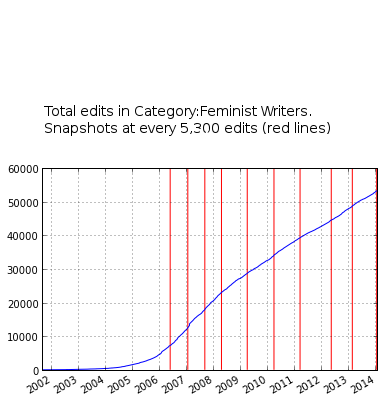
\includegraphics[width=0.9\columnwidth]{accumulative snapshot points for Feminist Writers.png}.
\caption{Matrix}
\label{fig:triangle_matrix}
\end{figure}


%Theory of ranking  \cite{Blumm2012}

%\subsection{criticism of alternative economy}
%we are not really saying much about how the economy of wikipedia, i.e. inputs and outputs.
%
%but still we can say something about the fact peer production, is indeed different from tradition economy.
%
%but still might be useful to justify why we are using HH model, and what we expect as differences. 

%\subsection{criticism of improving rankings approach}
%no reliable metrics for ranking people, there is never a benchmark to say that we have a "BETTER" metric in terms of measuring quality, precisely because we use those to calibrate.

%but still can say it is an effecient alternative metric, 

%\subsection{issue of possible overfitting}
%how do we justify the existence of alpha and beta as the parameters we calibrate

\section{Related Work}
To the best of our knowledge, our paper is the first attempt to quantify the structure and the impact of collaboration on value creation in open collaboration environments. Our model of {bi-partite random walkers} follows in the lineage of bi-partite networks -- with two node types -- in the global economy of countries competing for exporting products \cite{hidalgo2007,hidalgo2009}. The proposed {\it method of reflections} helps understand the competitive advantage (i.e., {\it fitness}) of countries from the types of products they sell, and moreover, whether other countries export similar products {\it ubiquity}. Most competitive countries are found to export non-ubiquitous products, for which they can charge higher price. The reflexive model has been iteratively improved and complemented in more recent work, mainly to fix the robustness of the method of reflections.\cite{tacchella2012new, cristelli2012competitors, tacchella2013economic, cristelli2013measuring}. Caldarelli et al. \cite{caldarelli2012network} have proposed an alternative method, based on biased Markov chains, which helps further understand the relations between two types of nodes in bi-partite networks. 

At the opposite of networks of economic competition, collaboration networks have been studied early on in network sciences, in particular networks of co-authorship in scientific publications \cite{newman2001}, as well as patterns of self-organization in bi-partite networks of actors-movies\cite{ramasco2004self}. Similarly, the analysis of patterns in the Wikipedia bi-partite networks confirmed the existence overlapping cliques of densely connected articles and editors  \cite{jesus2009}. In the same study, clustering of densely connected cliques into larger modules \cite{guimera2007module} showed that topics aggregate editors by interest with highly coordinated efforts in densely populated clusters \cite{jesus2009}.

In a series of Matlab contests aimed at collectively solving NP-hard problems, it was found that work shared as a public good helps individuals quickly reuse existing results, and thus, find better algorithms \cite{gulley2010}. Efforts have also been undertaken to assess the {\it expertise} of contributors \cite{geiger2013}, as well as the quality of articles \cite{wang2013tell} in Wikipedia.

\section{Method}
\label{method}
\textcolor{red}{Measuring the structure of value creation by individuals is nearly impossible in most in open collaboration projects.} In particular, when projects do not involve writing software code, they can hardly be compiled, executed and tested on computers. As exemplified in Wikipedia, the most common way to code knowledge is natural language (e.g. Chinese, English, Spanish, French, German), which can hardly be systematically tested for performance. Natural language is indeed the realm of subjective interpretation by humans. 

Here, we present a method to model \textcolor{red}{(measure?)} value creation and performance in such environments. This method neither relies on the content or on subjective metrics, such as the number of edits, nor on the number of bytes changed overall or per edit. We recognize that value can be brought by each editor, regardless of the frequency, or the length of her contributions \cite{}. Only the number and the expertise of editors bring value to an article \cite{wilkinson2007}.  And the expertise of editors can be measured from the number and the quality of articles they have modified at least once.

For that, we consider a simple input, which is a representation of the bi-partite network of editors and their contributions to articles.  Namely, let us consider a matrix $M_{ea}$ of all editors having contributed to a Wikipedia category of articles. $M_{ea}$ takes value $1$ if editor $e$ has edited article $a$, and $0$ otherwise. Note that $M_{ea}$ only shows which editors have ever touched an article. We convert to a binary categorical input for this matrix because of the precedent set in \cite{kane2011,keegan2012,geiger2013}, which each seek to move beyond the importance of edit count, claiming it to be spurious data when imagining the graph of editors, or measuring editor experience. For the category {\it Feminist Writers}, as presented on Figure \ref{fig:triangle}, $M_{ea}$ exhibits a triangular structure in which editors (resp. articles) are sorted (max on the bottom-left corner) by the number of articles they have touched (resp. by the number of editors who have touched each article). $M_{ea}$ is the only input of the {\it bi-partite random walker} model described thereafter, for recursively characterizing the structure and the value of contributions in open collaboration, through the evaluation of editor expertise and article quality.

\begin{figure*}[!t]
\centering
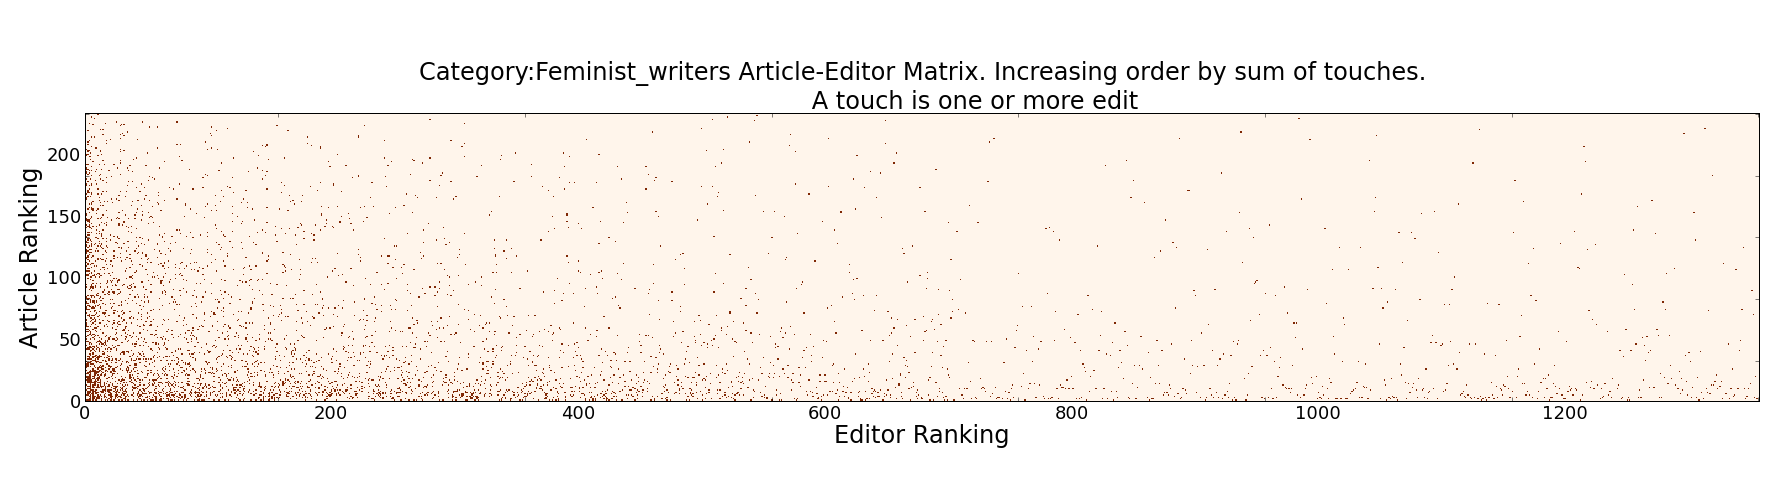
\includegraphics[width=2.0\columnwidth]{../Figures/Category_Feminist_writerstriangle_matrix_corrected.png}
\caption{Typical $\mathbf{\mathit{M_{ea}}}$ matrix for a Wikipedia category (here, {\it Feminist Writers}) ordered on both dimensions by descending order of number of articles modified by an editor (horizontal axis) and of number editors who have modified an article (vertical axis). The structure of $\mathbf{\mathit{M_{ea}}}$ is triangular and shows that some editors have a pervasive activity over articles, while most editors edit only a few. Similarly, some articles receive widespread attention by editors, while most articles are modified only by a few editors.}
\label{fig:triangle}
\end{figure*}


Given $M_{ea}$, the simplest way to assess the contribution value, the {\it expertise}, of an editor is obtained by summing the number of articles ever edited out of a set of articles. Similarly, a simple {\it quality} measure for an article is the sum of editors who have ever modified it, following the famous adage on open source development: ``Given enough eyeballs, all bugs are shallow" \cite{raymond1999}. These crude expertise and quality metrics for editors and articles, respectively  given by,

\begin{equation}
\begin{cases}
 u_{e}^{(0)} = \sum_{a=1}^{N_{a}} M_{ea} \equiv k_e\\[7pt]
 u_{a}^{(0)} = \sum_{e=1}^{N_{e}} M_{ea} \equiv k_a
\end{cases}
\label{HHinit}
\end{equation}

are the zero\textsuperscript{th} order of our algorithm. They are the initial step of the {\it method of reflections} proposed by Hidalgo et al. \cite{hidalgo2007,hidalgo2009}, which derives the value of producing entities (i.e. editors) from products (i.e. articles), and {\it vice versa}. To help capture the intuition behind the method of reflections for open collaboration, we walk through the first and second iterations:

\begin{itemize}
  \item {\bf 1\textsuperscript{st} order iteration,}  
  \begin{itemize}
  \item {\bf Articles}: If an article has been edited by higher expertise editors, it is of higher quality. That is, quality is a function of expertise calculated from zero\textsuperscript{th} iteration expertise scores.
  \item {\bf Editors}: Conversely, if an editor has contributed to higher quality articles, her expertise is higher. That is, expertise is a function of quality calculated from zero\textsuperscript{th} iteration quality scores.
  \end{itemize}
  \item {\bf 2\textsuperscript{nd} order iteration,}
    \begin{itemize}
  \item {\bf Articles}: If an article has been changed by higher expertise editors who have edited higher value articles, which in turn have been edited by higher expertise contributors, the article quality is higher. That is, quality is a function of expertise calculated from 1\textsuperscript{st} iteration expertise scores.
  \item {\bf Editors}: Conversely, if an editor has edited higher quality articles, which have been edited by better editors who have edited higher quality articles, then expertise is higher. That is, expertise is a function of quality calculated from 1\textsuperscript{st} iteration quality scores.
  \end{itemize}
 \item {\bf And so on, recursively.}\\
\end{itemize}

Although interpretation is difficult past the very first iteration steps, at each iteration, the algorithm incorporates additional information on the quality of the articles and expertise of editor from the neighboring nodes in the bi-partite network. The higher order iterations 
%of the method of reflections are written as,
%
%\begin{equation}
%\begin{cases}
% u_{e}^{(n+1)} = \frac{1}{k_{e}}\sum_{a=1}^{N_{a}} M_{ea} \, u_{a}^{n}\\[7pt]
% u_{a}^{(n+1)} = \frac{1}{k_{a}}\sum_{e=1}^{N_{e}} M _{ea}\, u_{e}^{n}\\
%\end{cases}
%\label{HHhigher}
%\end{equation}
%
% variable weights to the scores from the previous iteration
can be modeled as a Markov process of random walkers on a bi-partite network, jumping with some probability from one node type to another node type \cite{caldarelli2012network}. A schematic representation of the random walk process on a bi-partite network is depicted in Figure \ref{fig:jumpers}. \textcolor{red}{The intuition is the following: a random walker jumps with some probability from an editor to a given article (i.e. the editor's expertise is positively influenced by the article's quality), and with another probability from an article to a given editor (i.e. the value of the article is positively by the editor's expertise)}. The binary matrix $M_{ea}$ determines whether a jump between each pair of nodes is possible. If two nodes $e$ and $a$ are not directly connected $M_{ea} = 0$, and the transition probability is 0. Conceptually, the {\it bi-partite network random walker} model is an extension of the single node type (i.e. Web pages) {\it Page Rank} Google search algorithm \cite{page1999pagerank,kleinberg1999} to two kind of nodes.

\begin{figure}[!t]
\centering
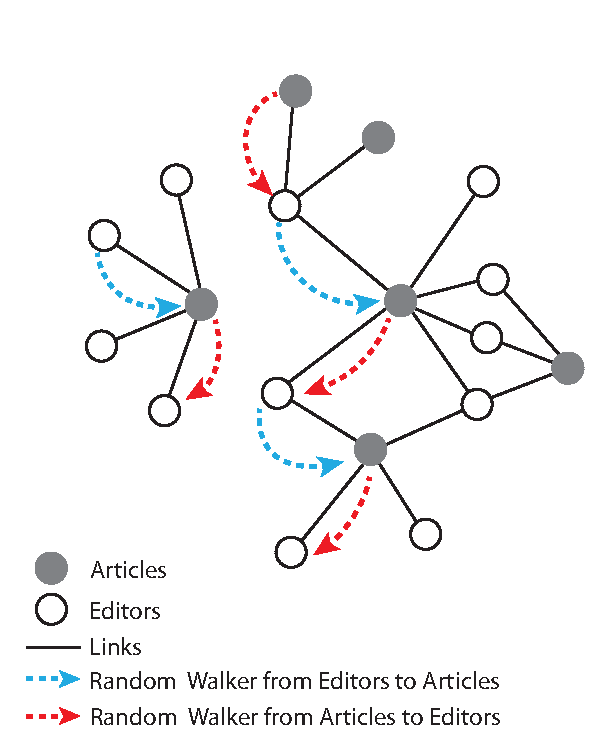
\includegraphics[width=0.7\columnwidth]{../Figures/bi-partite_net.eps}.
\caption{Representation of random walkers jumping from editors to articles (red dotted arrows) and from articles to editors (blue dotted arrows). The intuition is the following: a random walker jumps with some probability from an editor to a given article (i.e. the editor's expertise is positively influenced by the article's quality), and with another probability from an article to a given editor (i.e. the value of the article positively influences the editor's expertise).}
\label{fig:jumpers}
\end{figure}

%According to  Caldarelli et al. \cite{caldarelli2012network}, we reformulate the method of reflections to account for jumps of the random walker on the bi-partite network of editors and articles. 
We call $w^{(n)}_e$ the expertise of an editor and $w^{(n)}_a$ the quality of an article at the $n^{th}$ iteration, and we define the following Markov process on the bi-partite network of collaboration, 

\begin{equation}
\begin{cases}
w^{(n+1)}_e (\alpha,\beta) = \sum_{a=1}^{N_a}  G_{ea}(\beta) \,w^{(n)}_a (\alpha,\beta)\\[7pt]
w^{(n+1)}_a (\alpha,\beta) = \sum_{e=1}^{N_e}  G_{ae}(\alpha) \, w^{(n)}_e (\alpha,\beta)\\
\end{cases}
\label{random_walker}
\end{equation}

with $G_{ea}$ the probability  to jump from article $a$ to editor $e$ in a single step, and the probability $G_{ae}$ to jump from editor $e$ to article $a$ also in a single step. These transition probabilities are given by,

\begin{equation}
\begin{cases}
G_{ea}(\beta) = \frac{M_{ea} k_{e}^{-\beta}}{\sum_{e' = 1}^{N_e} M_{e'a} k_{e'}^{-\beta}}\\[10pt]
G_{ae}(\alpha) = \frac{M_{ea} k_{a}^{-\alpha}}{\sum_{a' = 1}^{N_a} M_{ea'} k_{a'}^{-\alpha}}.\\
 \end{cases}
\end{equation}

The transition matrices $G_{ea}(\beta)$ and $G_{ae}(\alpha)$ depend only on the initial conditions: the binary matrix $M_{ea}$, as well as $k_e$ and $k_a$ given by (\ref{HHinit}), and are controlled only by parameters $\alpha$ and $\beta$.  We shall therefore explain only how $\beta$ influences the probability to jump from an article to an editor (i.e. the value of the article positively influences the editor's expertise). For $\beta = 0$, we recover the zero\textsuperscript{th} order iteration (\ref{HHinit}). For $\beta > 0$, the probability to jump from article $a$ to editor $e$ is a power law function $\sim 1/k_{e}^{~\beta}$ of the sum of articles $k_{e}$  modified by editor $e$. Hence, the larger $k_{e}$, the lower the probability to jump from $a$ to $e$ relative to other editors. On the contrary, if $\beta < 0$ the probability to jump from an article to an editor is a positive function of the sum of articles modified by the editor. For $-1 < \beta < 0$, the function is concave, while for $\beta < -1$, the function is convex, which means that the more articles have been edited by the editor, the even more the positive influence on articles. In a nutshell, $\beta$ relates the amount of articles edited on the overall editor's expertise. %which in turn has an influence on each edited article (along with the influence of other editors).
If $\beta \gg 0$, the positive influence of the number of contributed articles on the editor's expertise decreases. If $\beta$ close to $0$, the number of contributed articles increases linearly the editor's expertise. The same considerations hold for $\alpha$ and the probability $G_{ae}(\alpha)$ to jump from an editor to an article (i.e. the expertise of the editor positively influences the quality of an article).

%After each iteration, we have expertise and quality scores, which allow for the ranking of editors and articles respectively. When the rankings for both editors and articles do not change in two successive iterations we consider that the {\it bi-partite network random walker} model has converged. We have verified that the method converges on all our 12 Wikipedia categories.  
Figure \ref{fig:convergence} shows the evolution of expertise $w_e$ ranked among editors having contributed to articles in the {\it Feminist Writers} category on Wikipedia for the set of control parameters $(\alpha,\beta) =(0, 0.72)$. We can see how the algorithm progressively ranks editors: some editors with initial low rank (i.e. with few articles edited), get a higher rank as more information is incorporated from neighboring nodes as the number of iterations increases. In that case ($\beta >0$), editors have edited and contributed to fewer, but higher quality articles (i.e. articles edited by more editors who have edited less articles). Similarly, some initially high ranked editors, gradually drop in the ranking. They have edited many, but lower quality articles. 

\begin{figure}[!t]
\centering
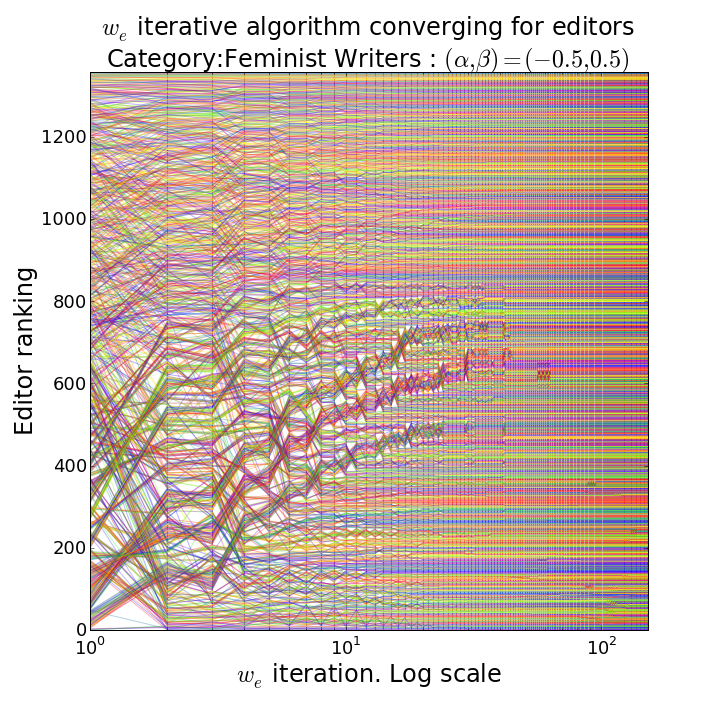
\includegraphics[width=0.9\columnwidth]{../Figures/fem_editors_iter_converge.png}.
\caption{Convergence of the ranked expertise $w_e$ of editors having contributed to articles in the Feminist Writers category on Wikipedia for arbitrary control parameters: $\mathbf{(\alpha,\beta) =(0, 0.72)}$. Starting from the sum of contributed articles as the initial step, we can see how the algorithm progressively ranks editors: some editors with initial lowest rank, i.e. with few articles edited, get a higher rank as the number of iterations increases. Similarly, some initially high ranked editors, gradually drop in the ranking. In the case {\it Feminist Writers}, the algorithm converges after $\mathbf{64}$ iterations.}
\label{fig:convergence}
\end{figure}

Upon calibration of the bi-partite random walker model with ground-truth metrics of article quality and editor expertise, the parameters $\alpha$ and $\beta$  directly informs how peer-production generates value through more broad collaboration (i.e. more articles edited by more editors), or on the contrary, more concentrated collaboration with small clusters of editors having touched less articles. 

% describe how editors and articles influence each other at the level of the whole bi-partite collaboration network.
%\textcolor{red}{We cannot calibrate and test because each category is different}


%Whenever calibration shows that the evolution of $\alpha$ and $\beta$ can be predicted, then editor expertise and article quality can also be predicted up to statistical errors. 
%Here, we explain the calibration steps for$\alpha$ and $\beta$ and how the control parameters inform on the structure of value creation in open collaboration. We also document the evolution of these parameters as Wikipedia categories get increasingly enriched with new contributions.

%A property of this algorithm, is that with the following balance condition,
%
%\begin{equation}
%\mathbf{G}_{ae} \mathbf{w}^*_e = \mathbf{G}_{ea} \mathbf{w}^*_a
%\end{equation}
%
%which can be rewritten as,
%
%\begin{equation}
%\begin{cases}
%\mathbf{w}^{*}_{e} \sim \mathbf{k}^{1-\beta}_{e} \langle \mathbf{k}_{a}^{-\alpha}\rangle_e \\
%\mathbf{w}^{*}_{a} \sim \mathbf{k}^{1-\alpha}_{a} \langle \mathbf{k}_{e}^{-\beta}\rangle_a
%\end{cases} \label{eqsim}
%\end{equation}
%
%it is the analytical formulation we use onwards. It is important to note a crucial difference in the way we apply the weighted random walk model in the case of open collaboration compared to the countries-products problem. In \cite{caldarelli2012network}, $w^*_p$ is a measure of ubiquity (i.e. dis-quality) because many countries can sell the product, while here $w^*_a$ is also a measure of ubiquity in the sense that many editors have modified the article. In the case of open collaboration, $w^*_a$ is a measure of quality.




%With some imagination Wikipedia, and many other online collaborative projects can be viewed as such a market. (Here we only consider English Wikipedia). We consider Wikipedia Editors to be our "countries", and Wikipedia Articles to be "products". Therefore a country producing a product is interpreted as an editor editing an article. We also inherit the assumption that the better editors will be those who edit the rarer articles, although we re-adjust that assumption in instructive ways later on. 


%2. We develop a new measure for the degree of collaborativity of category.

%Questions. Can this economics theory be applied, into other "economies"? Which is the other side of a Wikipedia question, which is "What are better ways to rank Wikipedia editor and articles, since the flawed Edit Counts and Article Metrics, are used as proxies"?


\section{Data}

%\subsection{Construction of Matrix $M$}
We seek to find values of $\alpha$ and $\beta$ that minimize the distance between rankings given by the bi-partite network random walker model, which takes the matrix $M$ as unique input, and ground-truth metrics on editor expertise and article quality, obtained independently from Wikipedia. We perform the model calibration for 13 snapshots (see Figure \ref{fig:snapshots})  for each of  the 12 categories of Wikipedia articles presented in Table \ref{tab:statistics}. For each category and snapshot, we build the binary matrix $M$ by parsing all edit histories of all articles up to the snapshot time. We set $M_{ea} = 1$ for editor $e$ having modified article $a$, and $M_{ea} = 0$ otherwise. In order to eliminate page vandals, we considered only editors who made 5 or more edits to any article in the category. We also discarded all software robots {\it Bots} that programmatically edit Wikipedia. 

\begin{table}
\begin{tabular}{|l|c|c|c|}
%\toprule
\hline
{\bf Category} &  {\bf Articles} &  {\bf Editors} &  {\bf Edits} \\
%\midrule
\hline
American male novelists               &      2,460 &   9,946 &  224,783 \\
2013 films                            &      1,896 &   5,215 &  150,956 \\
American women novelists              &      1,936 &   5,968 &  138,716 \\
Nobel Peace Prize laureates           &       104 &   4,165 &   91,522 \\
Sexual acts                           &        93 &   2,190 &   45,901 \\
Economic theories                     &       212 &   1,145 &   28,658 \\
Feminist writers                      &       233 &   1,357 &   25,738 \\
Yoga                                  &       123 &    730 &   25,315 \\
Military history of the US &       180 &    854 &   20,172 \\
Counterculture festivals              &        66 &    578 &   10,515 \\
Computability theory                  &        92 &    272 &    7,117 \\
Bicycle parts                         &        70 &    210 &    4,981 \\
\hline
\end{tabular}
\caption{Size statistics of investigated Wikipedia categories sorted by total edits.}
\label{tab:statistics}
\end{table}

\begin{figure}[!t]
\centering
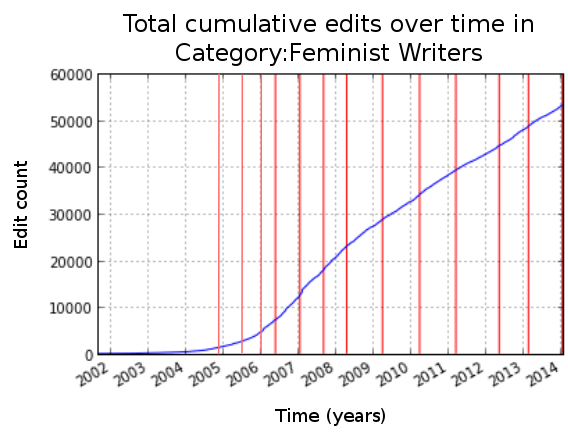
\includegraphics[width=0.9\columnwidth]{../Figures/cumulative_snapshots_Feminist_Writers_thirteen.png}
\caption{Cumulative edits made in Category {\it Feminist writers} (blue line). Vertical red lines represent the 13 snapshots taken at 2.5\%, 5\%, 7.5\% and then, 10\%, 20\%, 30\%, \ldots , 100\% of edits.}
\label{fig:snapshots}
\end{figure}

%\subsection{Editors Expertise and Articles Quality}
To calibrate $\alpha$ and $\beta$, we resorted to state-of-the-art ground-truth evaluations for editor expertise $\bar{w}_e$ and article quality $\bar{w}_a$. From these exogenous evaluations, we ranked editors and articles according to their expertise and quality respectively. We then performed  a grid search for values of $\alpha^*$ and $\beta^*$, which maximize the Spearman rank-correlation $\rho_e$ and $\rho_a$ between rankings obtained from the bi-partite random walker model $(w_e,w_a)$ and from exogenous metrics $(w_a,\bar{w}_a)$. Actually, $(\alpha^*,\beta^*)$ must maximize both $\rho_e$ and $\rho_a$, even though $\rho_e$ and $\rho_a$ might actually be different. The optimization function  of $(\alpha^*,\beta^*)$ is given by,

\begin{equation}
\begin{cases}
(\alpha^*,\beta^*) = argmax(\rho_e)\\
(\alpha^*,\beta^*) = argmax(\rho_a).\\
\end{cases}
\end{equation}
$(\alpha^*,\beta^*)$ characterize how value flows from editors to articles, and from articles to editors, in the bi-partite network of collaboration in Wikipedia.

According the ground-truth metrics, editor expertise is represented by labor hours, which have been  found as the most representative metric \cite{geiger2013}, and was calculated for each editor by taking contribution history up to the snapshot point. All edits made within 1 hour of a previous edit are counted in an {\it edit session}. If more than one hour separates two edits, a new period of edits  starts. The expertise expressed in labor hours is the sum of edit sessions. For the calculation of ground-truth expertise, we only consider edits for a given category, although the same editor might have edited other categories of articles in Wikipedia. Our measure of actual article quality is performed through a combination of 5 text analysis metrics: (i) ratio of mark-up to readable text, (ii) number of headings, (iii) article length, (iv) citations per article length, (v) outgoing intra-Wiki links. These metrics are used to determine quality on Wikipedia \cite{wang2013tell}, and have been widely tested \cite{klein}. We performed Principal Component Analysis (PCA) for each category and snapshot in order to reduce dimensionality from 5 metrics to a single one (i.e. the principal component). The variance explained by the principal component varied between 0.5 and 0.72, confirming the dominance of the axis of maximum variance.




\section{Results}
To understand how contributions by editors to articles shape the structure of collaboration in Wikipedia, we have performed a calibration of the bi-partite network random walker model on 12 Wikipedia categories (c.f. Table \ref{tab:statistics}) with 13 snapshots each (Figure \ref{fig:snapshots}). For each category and snapshot, we found the set of parameters $(\alpha^*,\beta^*)$, which maximize the fitness of the model to ground-truth metrics of article quality and editor expertise. Figure \ref{fig:landscape} shows typical optimization landscapes, which maximize the rank correlation $\rho_e$ (upper panel) between editor expertise $w_{e}$ obtained from the model and expertise obtained from state-of-the-art measures $\bar{w}_e$. The same is done for rank correlation $\rho_a$ between $w_a$ and $\bar{w}_a$ (lower panel). 

\begin{figure}[!t]
\centering
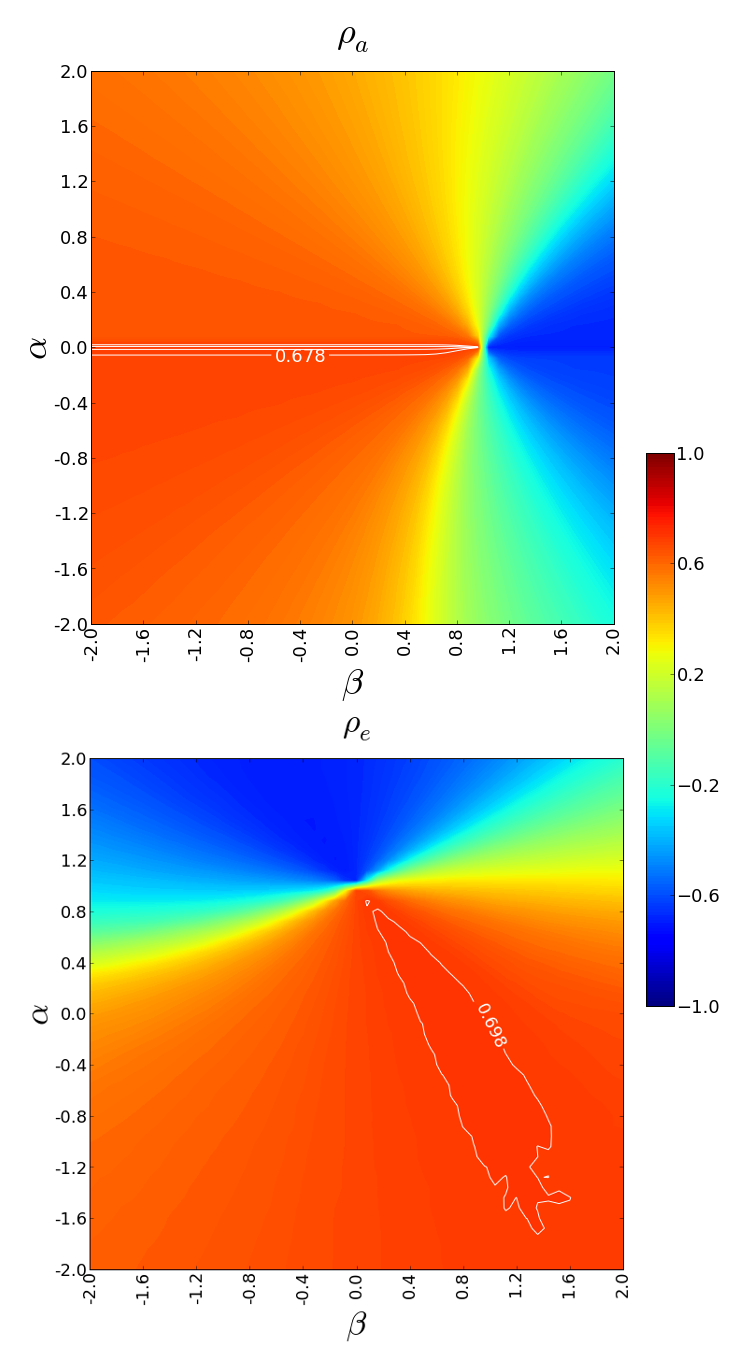
\includegraphics[width=0.9\columnwidth]{../Figures/contour_fem_combined.png}.
\caption{Typical landscape of maximum correlation as a function of $\alpha$ and $\beta$ for articles (upper panel) and editors (lower panel). The contour line shows the 95\textsuperscript{th} percentile of the rank correlation over the landscape. The category displayed here is {\it Feminist Writers}, for the last snapshot ending February 2014.}
\label{fig:landscape}
\end{figure}

The maximum achievable rank-correlation with ground-truth expertise and quality metrics for respectively editors \cite{geiger2013} and articles \cite{wang2013tell} shows that the bi-partite network random walker model accounts particularly well for both quality of articles ($0.58 < \rho_a < 0.91$) and expertise of editors ($0.46 < \rho_e < 0.75 $) at the last snapshot. Actually, the model reproduces very well, and very early the ranking of editors and articles according to the ground-truth metrics as shown on Figure \ref{fig:rhotime}. In particular, the quality of articles is very well accounted for, while the level of correlation with the ground-truth of editor expertise exhibits a slightly concave, or at least linear, increase.

%The question remains if the intersection of the solution spaces for $\rho_a$ and $\rho_e$ is nonempty. That is whether the we can find values of $\alpha$ and $\beta$ for which our editor ranking and article ranking are simultaneously optimized. We exploit two empirical facts from our data: the clear solution for article rankings that $alpha = 0$, and that for editor rankings the 95\textsuperscript{th} percentile maximizing boundary always includes values at $\alpha = 0$. Therefore, with $\alpha = 0$, we solve for $\beta$ in the editor ranking that maximizes $\rho_e$ - and thus $\rho_a$ simultaneously. 

For the latest snapshot (i.e. the state of contributions in February 2014), we find that the best possible $\alpha^*$ is $0$ in all circumstances, while $\beta^*$ varies considerably across categories. Table \ref{tab:maxbeta} shows the categories ordered by $\beta^*$ (and $\alpha^*=0$ for the sake of completeness), as well as the corresponding maximum rank correlations $\rho_e$ and $\rho_a$. Since there is no single optimal value for $(\alpha^*,\beta^*)$, but rather a space of optimal values for  $\rho_e$ and $\rho_a$ separately, we have searched for a set of values that jointly maximizes both $\rho_e$ and $\rho_a$. The optimal parameter $\alpha^* = 0$ means that editor expertise always benefits from contributions as a linear function of the number of articles edited [compounded over iterations of the recursive algorithm defined by formula (\ref{random_walker})].  However, $\beta^*$ exhibits a continuum of values between $0$ ({\it Bicycle parts} and {\it US Military History}) and $1.52$ ({\it Sexual Acts}). $\beta$ controls the influence of the number of editors on the quality of a given article. When $\beta \approx 0$, the quality of articles increases as a linear function of the number of editors who have modified them. For $\beta \gg 0$, the marginal gain of having more editors for a given article decreases. So, in that case, when the number of editors touching an article increases, the marginal quality improvement decreases.

The evolution of $\beta^{*}$ over snapshots as shown on Figure \ref{fig:rhotime} exhibits large variations for early snapshots corresponding to the early 10\% of overall contributions per category (i.e. the 4\textsuperscript{th} snapshot). While $\beta^{*}$ exhibits a tendency to more stability afterwards, large variations within the range $0$ to $1.5$ can be observed for some categories, suggesting that organization changes, along with the coordination level, can occur as categories further develop. 

%In fact, $\beta$ switches signs only 3 times of the possible 144 measured changes. Although there are not enough $\beta < 0$ to draw a firm conclusion, it is interesting to note that instances of $\beta < 0$ happened in early category history, hence suggesting that the early contributions steps pull more value from the community. 
%The stability of $(\alpha^*,\beta^*)$ confirms that the control parameters of the bi-partite network random walker model describe a robust feature of the structure of value creation in the bi-partite network of editors contributing to articles. This additional result is also a first step towards robust predictions of editor expertise and article quality rankings, given successive inputs to new articles made by editors.


\begin{table}
%\end{table}
\begin{tabular}{|llcccc|}
\hline
         &                     Category & $\rho_a$ & $\rho_e$ & $\alpha^{*}$ & $\beta^{*}$ \\
\hline
 1&                        Bicycle parts  &     0.90 &     0.46 &     0.00 &    0.00 \\
 2&Military history of the US  &     0.58 &     0.70 &     0.00 &    0.00 \\
  3&                Computability theory &     0.77 &     0.56 &     0.00 &    0.32 \\
   4&            American male novelists &     0.67 &     0.75 &     0.00 &    0.40 \\
    5&                        2013 films  &     0.72 &     0.55 &     0.00 &    0.48 \\
     6&                Economic theories  &     0.74 &     0.70 &     0.00 &    0.48 \\
     7&         American women novelists  &     0.63 &     0.75 &     0.00 &    0.64 \\
     8&                 Feminist writers  &     0.70 &     0.69 &     0.00 &    0.72 \\
     9&                             Yoga  &     0.64 &     0.57 &     0.00 &    1.12 \\
     10&      Nobel Peace Prize laureates  &     0.91 &     0.66 &     0.00 &    1.20 \\
      11&        Counterculture festivals  &     0.80 &     0.61 &     0.00 &    1.36 \\
        12&                   Sexual acts  &     0.63 &     0.66 &     0.00 &    1.52 \\
\hline
\end{tabular}
\caption{Categories ordered by increasing $\beta^{*}$ obtained from best rank-correlation $\rho_a$ and  $\rho_e$
 of the {bi-partite network random walker} with the ground truth. As shown on the upper panel of Figure \ref{fig:landscape}, highest rank-correlation is always obtained for $\alpha^{*} = 0$ suggesting that editors are experts in direct proportion to the number of articles they edit. The different values of $\beta^{*}$ show the effect of marginal editors on a article. As $\beta^{*}$ grows larger having more editors shows diminishing returns on article quality - ``too many cooks spoil the broth".}
\label{tab:maxbeta}
\end{table}


%However, for categories with $\beta >0$ the quality of an article is also negatively influenced by the portfolio size of its editors. In other words, when $\beta$ is large, the more articles an editor edits, the lower his or her contributed value to one single article. $\beta$ also characterizes each category and the way quality is achieved through the cumulative contribution of information. For $\beta$ small, all editors have a fairly equal chance to contribute positively to any article, while for $\beta$ large, an editor can only contribute positively to a subset of articles (the larger $\beta$ the smaller the set). Typically, it is unlikely for a single person to have visited all {\it counterculture festivals}, performed all {\it sexual acts} or {\it Yoga} practices, while it is easier for anyone to gather relevant information on {\it bicycle parts} or the {\it US military history}. 





%\textcolor{red}{\bf Is there any reshuffling of ranking over time, or do they stay the same?}



\begin{figure}[!t]
\centering
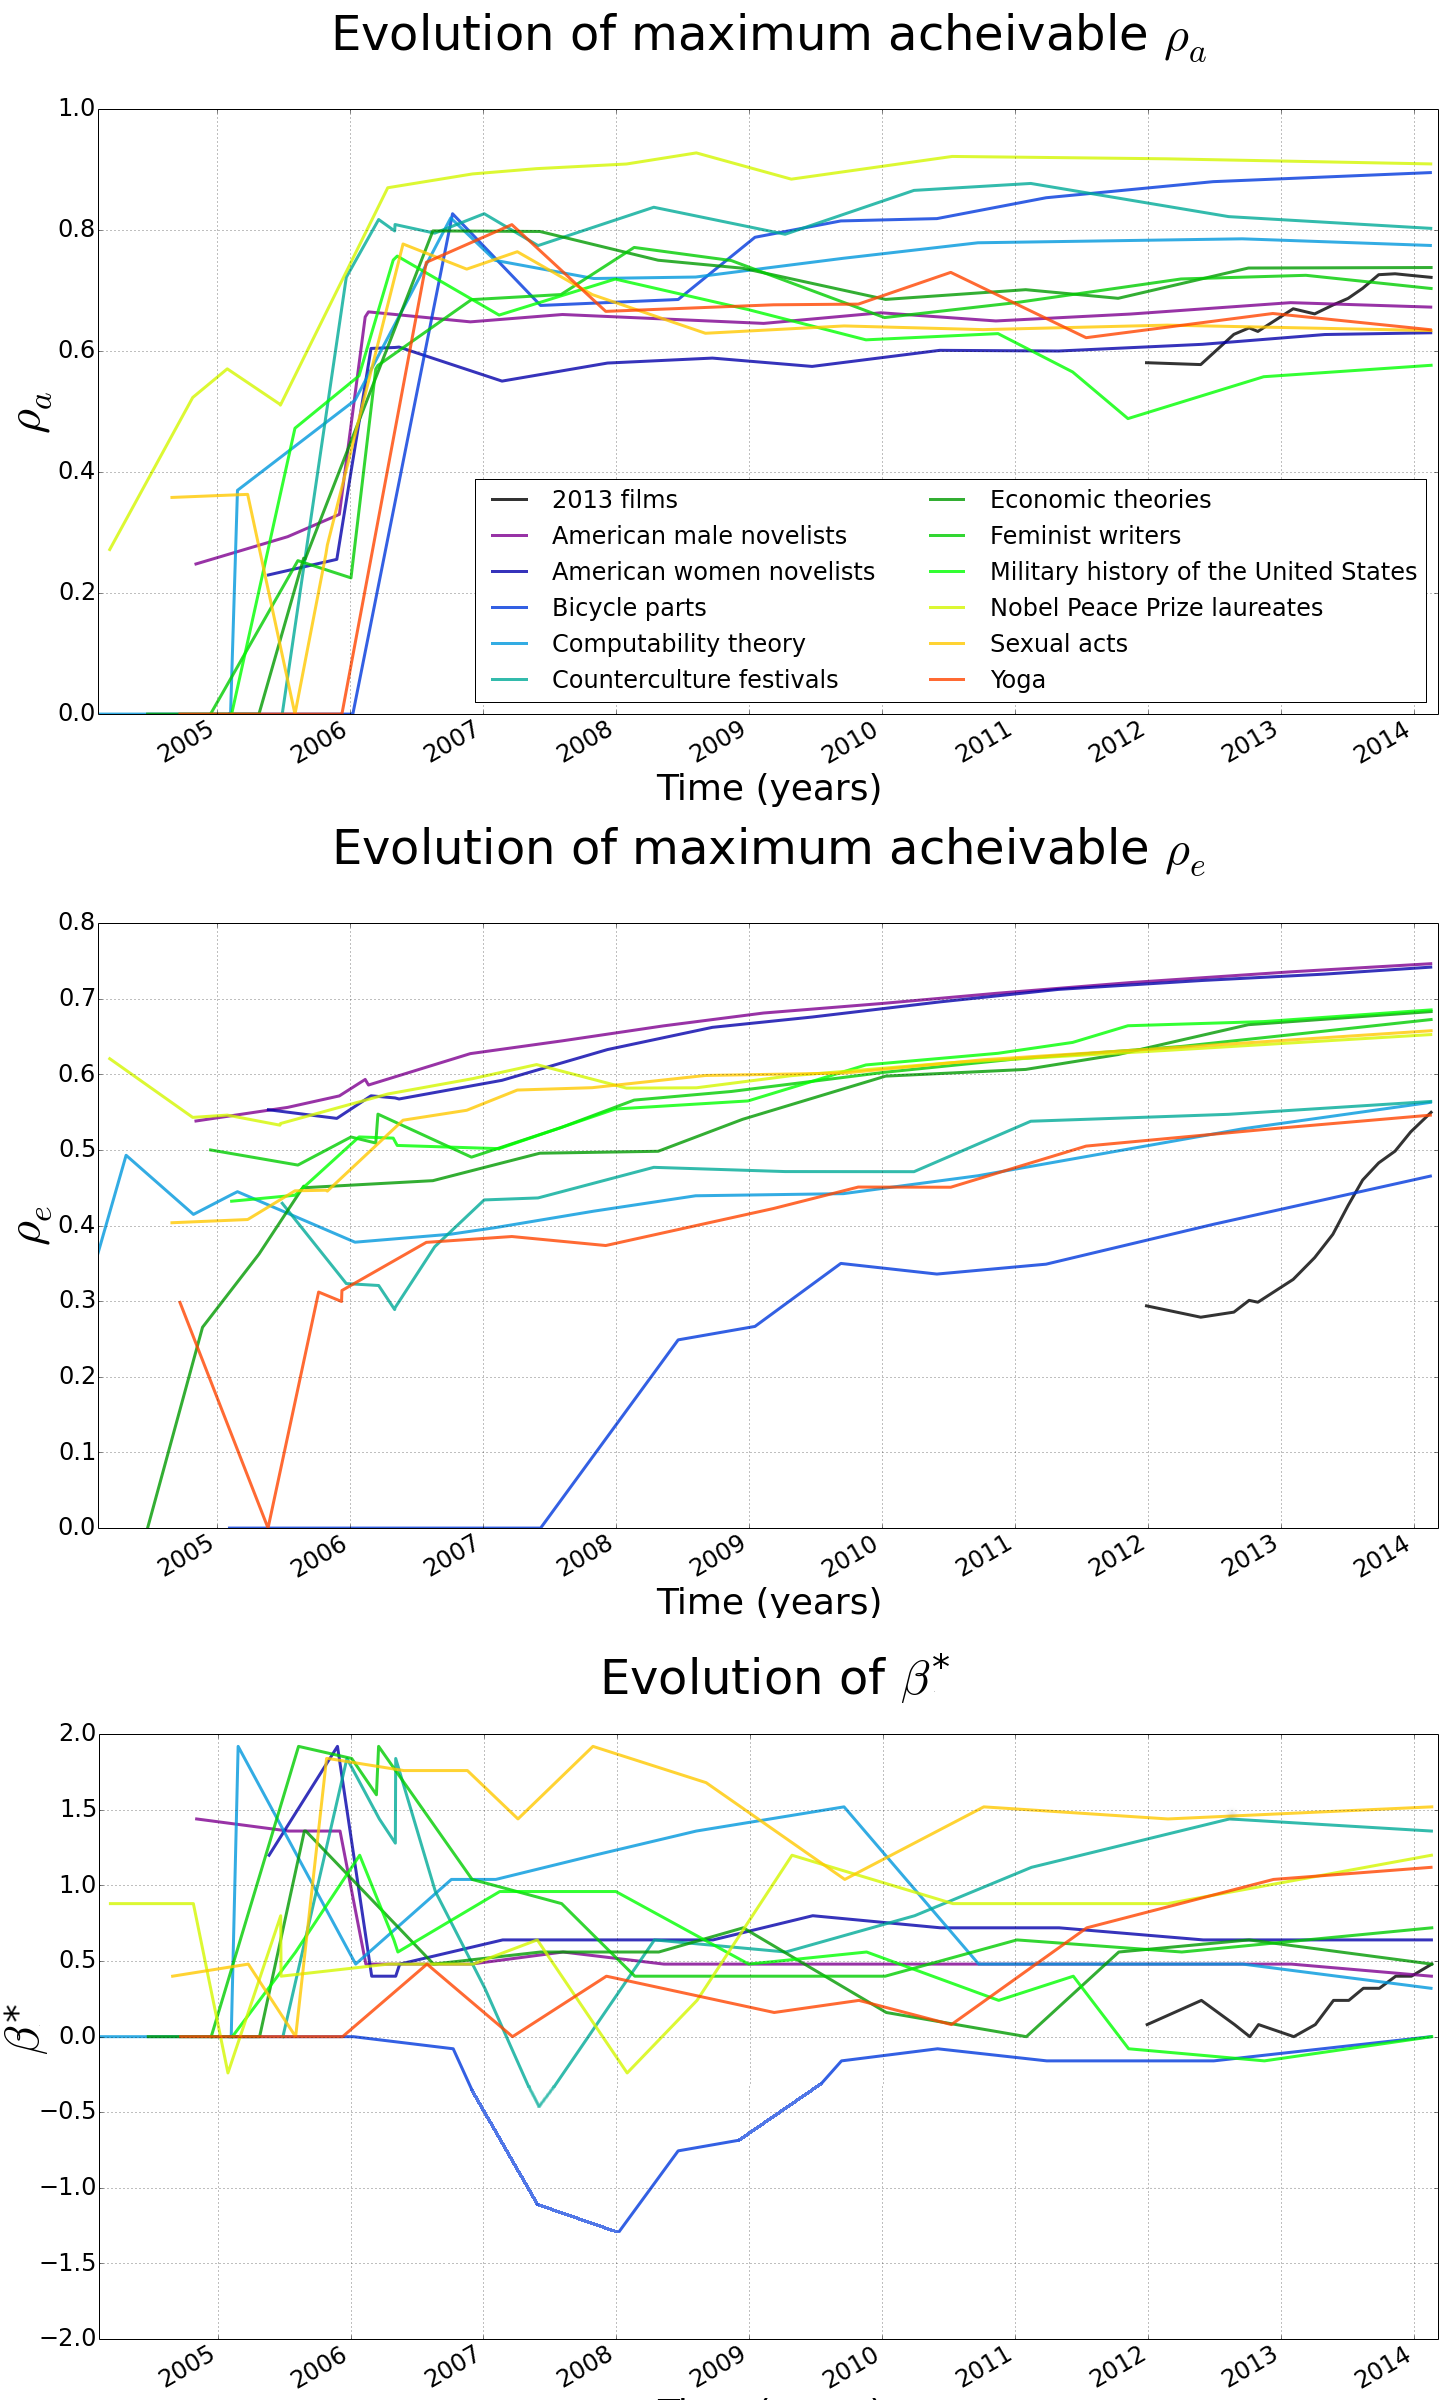
\includegraphics[width=0.9\columnwidth]{../Figures/rho_combined_with_beta.eps}.
\caption{Evolution of Spearman $\rho$ rank correlations between the ranking obtained from the calibrated model and the actual values for each category and for editors (upper panel)  and articles (middle panel). Corresponding $\beta^{*}$ values are also shown for interest (lower panel). The correlations are generally quite high : $ 0.46 < \rho_e < 0.75$ with $\langle \rho_e\rangle = 0.64$ for editors and $0.57 < \rho_a < 0.91$ with $\langle \rho_a\rangle = 0.72$. $\rho_{a}$  is stable over time, which means that the quality of articles can be well captured early on by the model. However, $\rho_e$ exhibits a convex increase over time, suggesting that it takes time (i.e. lots of edits) to capture well the expertise of editors.}
\label{fig:rhotime}


\end{figure}

	






\section{Discussion}
Building on the method of reflections previously used for global economic networks of production, we have applied and tested the {\it bi-partite network random walker} model in the context of Wikipedia open collaboration. Our results show that the model accounts well for the quality of articles  $\langle \rho_a \rangle  \approx 0.64$ and for the expertise of contributors $\langle \rho_e \rangle  \approx 0.72$. Moreover, the evolution of $\rho_e$ and $\rho_a$ of categories under editing, exhibit strong stability. In particular, the adequacy of article ranking is very high early on, and thereafter stationary, suggesting that the model can quickly capture the quality of articles. For editor expertise, the adequacy increases steadily as categories get further developed. 

This difference might be due to the roughness of the actual metrics for editors $\bar{w}_e$, expressed in labor-hours, compared to the quality of $\bar{w}_a$, which is an aggregate measure of five precise quality metrics. Nevertheless, the correlation of editor ranking with $\bar{w}_e$ increases: $\rho_e$ exhibits a convex increase over time, suggesting that it takes time (i.e. lots of articles edited) to capture well the expertise of editors. This is striking because the method is reflexive and the same information is incorporated on both dimensions from the input matrix $\mathbf{\mathit{M}}$. While it will require further investigation to explain, we interpret this result in the following way: from Figure \ref{fig:triangle} and from Table \ref{tab:statistics}, we see that there are always significantly more editors than articles for each category. This means that the probability for an article to get contributions early on is higher than the probability to find editors who have contributed to a lot of articles early. In other words, it takes more time to correctly rank editors because there are more editors compared to the number of articles in a given category.

%We have also found $\alpha \approx 0$ for all categories, reflecting the positive influence of the number of articles edited on editor expertise. This fact tells actually a lot about the model.  The actual metric for editor expertise takes only into consideration the labor hours \cite{geiger2013}, and the more time is spent editing a category, the more likely the editor will have modified a large quantity of articles. The value of $\alpha$ can therefore be explained entirely by the nature of the ground-truth metric. Although it would require further testing with a broad variety of metrics, it seems that the {bi-partite network random walker} model can {\it tune} to whatever ground-truth metric used for calibration. In other words, the values of $\alpha$ and $\beta$ only reflect the structure of value creation in open collaboration, {\it given} the chosen ground-truth metrics. 

We have also found $\alpha \approx 0$ for all categories. This result shares similarity  with \cite{keegan2012}, who found that "editor experience and the features of articles in their contribution history have a stronger influence on self-organization than article features and the attributes of their editors". In this way if editor expertise is more important, it makes sense that we find it, $\alpha$, to be a near-constant (although that doesn't explain why it should be zero). Allowing for a moment, $\alpha = 0$ we can simplify our analytic solutions to gain a more intuitive interpretation of the calibration results.

\begin{equation}
\begin{cases}
 w^{*}_{e} \sim k_{e}^{1-\beta}\langle k_{a}^{-\alpha} \rangle_{e}\\[7pt]
 w^{*}_{a} \sim k_{a}^{1-\alpha}\langle k_{e}^{-\beta} \rangle_{a}\\[7pt]
\end{cases}
\end{equation}


Then letting $\alpha = 0$, we can simplify to:
\begin{equation}
\begin{cases}
 w^{*}_{e} \sim k_{e}^{1-\beta}\\[7pt]
 w^{*}_{a} \sim k_{a}
 \langle k_{e}^{-\beta} \rangle_{a}\\[7pt]
\end{cases} 
\end{equation}
 
 Recalling that the variables $\alpha$ and $\beta$ control the preferential attachment to move to more connected editor or article nodes in the transition matrix. We will talk about the importance of "super-users" and "super-articles" as those nodes nodes that would be effected greatly by preferential attachment.  We concentrate on our unfix variable, $\beta$, as it influences editor ranking \ref{fig:influence_editors} and article ranking.\ref{fig:influence_artilces}. Over all categories and snapshots we found $-2 < \beta < 2$, which has a related spectrum of interpretations. With examples from both ends of the spectrum we find footing to consider $\beta$ as a proxy for ``collaborativeness". 
 
Consider the highest $\beta$ found, on category {\it Sexual acts}. We chose to include this category because it could be considered taboo or perverse to edit these articles.  This category's articles are the least collaboratively edited; the high $beta > 1$ means that many edits - albeit very slightly - hurt your ranking does \ref{fig:influence_editors}. While this may seem counter intuitive, an explanation can be seen through the fact that Wikipedia is notable for a vast and constant amount of vandalism and "edit-warring", which often has a juvenile and lewd nature. Previous Wikipedia research has shown this unintuitive result, that on some articles most active editors exhibit deleting behavior that would lower metric-based article quality ratings \cite{kane2011}. Articles about Sexual Acts, because of their socially-sensitive nature are particularly prone to attracting vandals or edit-warring behavior. Therefore the editors making the most edits are not necessarily the ones improving article quality, as we would typically expect.

This category is at the chaotic end of the Wikipedia spectrum. On the other hand, there are more prime examples of organized activity. Category {\it Military History of the US} is famous within Wikipedia for its self-organizing task-forces, and at the latest snapshot exhibits $\beta = 0$. In fact, it is the only Category that ever have consecutive snapshots where a maximal correlation came from $\beta < -1$. The interpretation of $\beta < -1$ is that article quality is very positively proportional to the number of editors touching the article \ref{fig:influence_artilces}. This is no coincidence, we chose this category, because it has a reputation for being very organized. Military History is a "WikiProject" with a hierarchy of coordinators, an IRC channel, and a mailing list. As a result of the coordination there is less edit-warring and more focused attention in the category. Each visit to the page by good editors has a definite, productive task at hand. This can also be seen by the $\beta \leq 0$ editor influence \ref{fig:influence_editors}, that super-users are linearly or super-linearly rewarded in rank for their contributions. It requires a frictionless, collaborative environment where the more you edit, the more and more experienced you become. It's also worth noting that \cite{keegan2012}, found that "coordination demands influence the tendency of editors with similar levels of experience to work together". In our scenario that would mean that the coordination present attracts super-users to work in the productive environment. The category Military History is empirically a standout case of collaboration, and shows in its calibrated $\beta$ measurements. 

That fact that we find two very different cases of collaborativeness is important in explaining previous contention in computer support collaborative work sphere. Early on research was release to suggest that high editor inequality among editors is related to high article quality \cite{kittur08}. The intuition is that the top superusers can be unrivaled in shaping the articles. We have certainly found this to be true in the Military History example. Yet later, it was found that editor inequality relating to article quality is unsupported, and editor inequality relating to coordination is false \cite{arazy}. In the case of chaotic categories like Sexual Acts we found this case, where the top users cannot make as much a positive impact as otherwise. These two seemingly contradictory findings can be explained through our measure of collaborativeness. Each part of wikipedia can exhibit different and measurable relationships between editor quality and article quality - that is our collaborativeness \beta. 

%$\mathbf{M}$ : most basic measure of collaboration, which represents the bi-partite network contributions to articles by editors: Here, we consider the simplest information available on collaboration: has an editor modified an article at any point in time or not ?


%Analyzing the Creative Editing Behavior of Wikipedia Editors: Through Dynamic Social Network Analysis \footnote{This paper analyzes editing patterns of Wikipedia contributors using dynamic social network analysis. We have developed a tool that converts the edit flow among contributors into a temporal social network. We are using this approach to identify the most creative Wikipedia editors among the few thousand contributors who make most of the edits amid the millions of active Wikipedia editors. In particular, we identify the key category of �coolfarmers�, the prolific authors starting and building new articles of high quality. Towards this goal we analyzed the 2580 featured articles of the English Wikipedia where we found two main article types: (1) articles of narrow focus created by a few subject matter experts, and (2) articles about a broad topic created by thousands of interested incidental editors. We then investigated the authoring process of articles about a current and controversial event. There we found two types of editors with different editing patterns: the mediators, trying to reconcile the different viewpoints of editors, and the zealots, who are adding fuel to heated discussions on controversial topics. As a second category of editors we look at the �egoboosters�, people who use Wikipedia mostly to showcase themselves. Understanding these different patterns of behavior gives important insights about the cultural norms of online creators. In addition, identifying and policing egoboosters has the potential to increase the quality of Wikipedia. People best suited to enforce culture-compliant behavior of egoboosters through exemplary behavior and active intervention are the highly regarded coolfarmers introduced above. }\cite{iba2010}


%{\bf Network Analysis of Collaboration Structure in Wikipedia} \footnote{In this paper we give models and algorithms to describe and analyze the collaboration among authors of Wikipedia from a network analytical perspective. The edit network encodes who interacts how with whom when editing an article; it significantly extends previous network models that code author communities in Wikipedia. Several characteristics summarizing some aspects of the organization process and allowing the analyst to identify certain types of authors can be obtained from the edit network. Moreover, we propose several indicators characterizing the global network structure and methods to visualize edit networks. It is shown that the structural network indicators are correlated with quality labels of the associated Wikipedia articles.} \cite{brandes2009}


%The problem of ranking entities and their respective production is relevant to the flourishing production of knowledge on the Web, and is directly related to two outstanding problems, which have been previously debated. First, how do we gauge the quality (resp. reliability) of blog posts, book reviews (e.g. on Amazon), or restaurant reviews (e.g. on Yelp) ?  Second,  how to grant editing and administrative privileges on community networks (e.g. Slashdot) and on online collaborative platforms (e.g. Wikipedia) \cite{halfaker2013}. 


\section{Limitations}
\label{limitations}
We do not directly measure the {\it capabilities} of editors. For instance, what does one editor do best to improve an article, among the five metrics (ratio of mark-up to readable text, number of headings, article length, citations per article length, and outgoing intrawiki links) we have used to assess the quality of an article ? 

We have not looked at the evolution of the quality of correlation as a function of iteration steps.

``less is more" : Why is it that when we incorporate more information in the matrix M, the results are not better ? Here we took the most simple metric (unlike HH method).

Quality of the exogenous metrics, especially for editors. It would be definitely make to look at real capabilities.

We only look at the ranking not at the real quality/expertise values ? Can we learn more the real values about the gap between articles/editors ?



\section{Discussion}
Building on the method of reflections previously used for global economic networks of production, we have applied and tested the {\it bi-partite network random walker} model in the context of Wikipedia open collaboration. Our results show that the model accounts well for the quality of articles  $\langle \rho_a \rangle  \approx 0.64$ and for the expertise of contributors $\langle \rho_e \rangle  \approx 0.72$. Moreover, the evolution of $\rho_e$ and $\rho_a$ of categories under editing, exhibit strong stability. In particular, the adequacy of article ranking is very high early on, and thereafter stationary, suggesting that the model can quickly capture the quality of articles. For editor expertise, the adequacy increases steadily as categories get further developed. 

This difference might be due to the roughness of the actual metrics for editors $\bar{w}_e$, expressed in labor-hours, compared to the quality of $\bar{w}_a$, which is an aggregate measure of five precise quality metrics. Nevertheless, the correlation of editor ranking with $\bar{w}_e$ increases: $\rho_e$ exhibits a convex increase over time, suggesting that it takes time (i.e. lots of articles edited) to capture well the expertise of editors. This is striking because the method is reflexive and the same information is incorporated on both dimensions from the input matrix $\mathbf{\mathit{M}}$. While it will require further investigation to explain, we interpret this result in the following way: from Figure \ref{fig:triangle} and from Table \ref{tab:statistics}, we see that there are always significantly more editors than articles for each category. This means that the probability for an article to get contributions early on is higher than the probability to find editors who have contributed to a lot of articles early. In other words, it takes more time to correctly rank editors because there are more editors compared to the number of articles in a given category.

%We have also found $\alpha \approx 0$ for all categories, reflecting the positive influence of the number of articles edited on editor expertise. This fact tells actually a lot about the model.  The actual metric for editor expertise takes only into consideration the labor hours \cite{geiger2013}, and the more time is spent editing a category, the more likely the editor will have modified a large quantity of articles. The value of $\alpha$ can therefore be explained entirely by the nature of the ground-truth metric. Although it would require further testing with a broad variety of metrics, it seems that the {bi-partite network random walker} model can {\it tune} to whatever ground-truth metric used for calibration. In other words, the values of $\alpha$ and $\beta$ only reflect the structure of value creation in open collaboration, {\it given} the chosen ground-truth metrics. 

We have also found $\alpha \approx 0$ for all categories. This result shares similarity  with \cite{keegan2012}, who found that "editor experience and the features of articles in their contribution history have a stronger influence on self-organization than article features and the attributes of their editors". In this way if editor expertise is more important, it makes sense that we find it, $\alpha$, to be a near-constant (although that doesn't explain why it should be zero). Allowing for a moment, $\alpha = 0$ we can simplify our analytic solutions to gain a more intuitive interpretation of the calibration results.

\begin{equation}
\begin{cases}
 w^{*}_{e} \sim k_{e}^{1-\beta}\langle k_{a}^{-\alpha} \rangle_{e}\\[7pt]
 w^{*}_{a} \sim k_{a}^{1-\alpha}\langle k_{e}^{-\beta} \rangle_{a}\\[7pt]
\end{cases}
\end{equation}


Then letting $\alpha = 0$, we can simplify to:
\begin{equation}
\begin{cases}
 w^{*}_{e} \sim k_{e}^{1-\beta}\\[7pt]
 w^{*}_{a} \sim k_{a}
 \langle k_{e}^{-\beta} \rangle_{a}\\[7pt]
\end{cases} 
\end{equation}
 
 Recalling that the variables $\alpha$ and $\beta$ control the preferential attachment to move to more connected editor or article nodes in the transition matrix. We will talk about the importance of "super-users" and "super-articles" as those nodes nodes that would be effected greatly by preferential attachment.  We concentrate on our unfix variable, $\beta$, as it influences editor ranking \ref{fig:influence_editors} and article ranking.\ref{fig:influence_artilces}. Over all categories and snapshots we found $-2 < \beta < 2$, which has a related spectrum of interpretations. With examples from both ends of the spectrum we find footing to consider $\beta$ as a proxy for ``collaborativeness". 
 
Consider the highest $\beta$ found, on category {\it Sexual acts}. We chose to include this category because it could be considered taboo or perverse to edit these articles.  This category's articles are the least collaboratively edited; the high $beta > 1$ means that many edits - albeit very slightly - hurt your ranking does \ref{fig:influence_editors}. While this may seem counter intuitive, an explanation can be seen through the fact that Wikipedia is notable for a vast and constant amount of vandalism and "edit-warring", which often has a juvenile and lewd nature. Previous Wikipedia research has shown this unintuitive result, that on some articles most active editors exhibit deleting behavior that would lower metric-based article quality ratings \cite{kane2011}. Articles about Sexual Acts, because of their socially-sensitive nature are particularly prone to attracting vandals or edit-warring behavior. Therefore the editors making the most edits are not necessarily the ones improving article quality, as we would typically expect.

This category is at the chaotic end of the Wikipedia spectrum. On the other hand, there are more prime examples of organized activity. Category {\it Military History of the US} is famous within Wikipedia for its self-organizing task-forces, and at the latest snapshot exhibits $\beta = 0$. In fact, it is the only Category that ever have consecutive snapshots where a maximal correlation came from $\beta < -1$. The interpretation of $\beta < -1$ is that article quality is very positively proportional to the number of editors touching the article \ref{fig:influence_artilces}. This is no coincidence, we chose this category, because it has a reputation for being very organized. Military History is a "WikiProject" with a hierarchy of coordinators, an IRC channel, and a mailing list. As a result of the coordination there is less edit-warring and more focused attention in the category. Each visit to the page by good editors has a definite, productive task at hand. This can also be seen by the $\beta \leq 0$ editor influence \ref{fig:influence_editors}, that super-users are linearly or super-linearly rewarded in rank for their contributions. It requires a frictionless, collaborative environment where the more you edit, the more and more experienced you become. It's also worth noting that \cite{keegan2012}, found that "coordination demands influence the tendency of editors with similar levels of experience to work together". In our scenario that would mean that the coordination present attracts super-users to work in the productive environment. The category Military History is empirically a standout case of collaboration, and shows in its calibrated $\beta$ measurements. 

That fact that we find two very different cases of collaborativeness is important in explaining previous contention in computer support collaborative work sphere. Early on research was release to suggest that high editor inequality among editors is related to high article quality \cite{kittur08}. The intuition is that the top superusers can be unrivaled in shaping the articles. We have certainly found this to be true in the Military History example. Yet later, it was found that editor inequality relating to article quality is unsupported, and editor inequality relating to coordination is false \cite{arazy}. In the case of chaotic categories like Sexual Acts we found this case, where the top users cannot make as much a positive impact as otherwise. These two seemingly contradictory findings can be explained through our measure of collaborativeness. Each part of wikipedia can exhibit different and measurable relationships between editor quality and article quality - that is our collaborativeness \beta. 

%$\mathbf{M}$ : most basic measure of collaboration, which represents the bi-partite network contributions to articles by editors: Here, we consider the simplest information available on collaboration: has an editor modified an article at any point in time or not ?


%Analyzing the Creative Editing Behavior of Wikipedia Editors: Through Dynamic Social Network Analysis \footnote{This paper analyzes editing patterns of Wikipedia contributors using dynamic social network analysis. We have developed a tool that converts the edit flow among contributors into a temporal social network. We are using this approach to identify the most creative Wikipedia editors among the few thousand contributors who make most of the edits amid the millions of active Wikipedia editors. In particular, we identify the key category of �coolfarmers�, the prolific authors starting and building new articles of high quality. Towards this goal we analyzed the 2580 featured articles of the English Wikipedia where we found two main article types: (1) articles of narrow focus created by a few subject matter experts, and (2) articles about a broad topic created by thousands of interested incidental editors. We then investigated the authoring process of articles about a current and controversial event. There we found two types of editors with different editing patterns: the mediators, trying to reconcile the different viewpoints of editors, and the zealots, who are adding fuel to heated discussions on controversial topics. As a second category of editors we look at the �egoboosters�, people who use Wikipedia mostly to showcase themselves. Understanding these different patterns of behavior gives important insights about the cultural norms of online creators. In addition, identifying and policing egoboosters has the potential to increase the quality of Wikipedia. People best suited to enforce culture-compliant behavior of egoboosters through exemplary behavior and active intervention are the highly regarded coolfarmers introduced above. }\cite{iba2010}


%{\bf Network Analysis of Collaboration Structure in Wikipedia} \footnote{In this paper we give models and algorithms to describe and analyze the collaboration among authors of Wikipedia from a network analytical perspective. The edit network encodes who interacts how with whom when editing an article; it significantly extends previous network models that code author communities in Wikipedia. Several characteristics summarizing some aspects of the organization process and allowing the analyst to identify certain types of authors can be obtained from the edit network. Moreover, we propose several indicators characterizing the global network structure and methods to visualize edit networks. It is shown that the structural network indicators are correlated with quality labels of the associated Wikipedia articles.} \cite{brandes2009}


%The problem of ranking entities and their respective production is relevant to the flourishing production of knowledge on the Web, and is directly related to two outstanding problems, which have been previously debated. First, how do we gauge the quality (resp. reliability) of blog posts, book reviews (e.g. on Amazon), or restaurant reviews (e.g. on Yelp) ?  Second,  how to grant editing and administrative privileges on community networks (e.g. Slashdot) and on online collaborative platforms (e.g. Wikipedia) \cite{halfaker2013}. 


\section{Limitations}
\label{limitations}
We do not directly measure the {\it capabilities} of editors. For instance, what does one editor do best to improve an article, among the five metrics (ratio of mark-up to readable text, number of headings, article length, citations per article length, and outgoing intrawiki links) we have used to assess the quality of an article ? 

We have not looked at the evolution of the quality of correlation as a function of iteration steps.

``less is more" : Why is it that when we incorporate more information in the matrix M, the results are not better ? Here we took the most simple metric (unlike HH method).

Quality of the exogenous metrics, especially for editors. It would be definitely make to look at real capabilities.

We only look at the ranking not at the real quality/expertise values ? Can we learn more the real values about the gap between articles/editors ?



\section{Conclusion}
We have presented a recursive algorithm based on a {\it bi-partite network random walker} model, which jointly ranks Wikipedia editors by their expertise, and articles by their quality, from a simple input matrix recording which editor has modified a given article. Moreover, upon calibration on 12 categories of Wikipedia articles, the input and the control parameters of the model inform directly on how value is created from the complex network of contributions. It appears that some categories of Wikipedia articles fully benefit from the multiplicity of contributors (i.e. ``collaborativeness"), while for other categories, more contributors per article generate dis-value. The origins of these differences between categories could stem from limited coordination capacity between contributors. The organization of value creation in open collaboration might also be intrinsically different from one topic to another. Finally, we want to stress the generality of the method we have presented. Similarly to open collaboration in Wikipedia, the proposed algorithm can be applied to a variety of situations, such as social coding (e.g. Github) , or collaborative rating (e.g. Amazon or Yelp reviews). By applying the algorithm in many domains we further understand to origins of collective value creation and quality, which are the hallmark of open collaboration.



%For each snapshot, we constructed the matrix $\mathbf{M_{e,a}}$ of contributors versus edited articles, similar to the country versus products matrix of the Economics Domain. For each snapshot, the values in $\mathbf{M_{e,a}}$ are defined as the number of edits made by editor $e$ on article $a$ in the category occurring in the snapshot time. Note that the final snapshot represents the entire history of the category up to the present date. 

%\subsection{Interpretation of w* algorithm in the context of open collaboration}
%
%To understand the results, we must have a firm grasp on what $\alpha$ and $\beta$ mean. They are more easily understood by roughly rewriting $\mathbf{w^*}$ as:
%\begin{equation}
%\begin{cases}
%w^{*}_{e} \sim k^{1-\beta}_{e} \langle k_{a}^{-\alpha}\rangle_e \\
%
%w^{*}_{a} \sim k^{1-\alpha}_{a} \langle k_{e}^{-\beta}\rangle_a
%\end{cases}
%\end{equation}
%
%where $\langle k_{a}^{-\alpha}\rangle_e$ is the arithmetic average of k  $k_{a}^{-\alpha}$. 
%
%Since we see beta and alpha are close to being additive inverses, we can just study what it means for them to increase and decrease.
%
%For Editors.
%As beta approaches one from infinity then editors are less judge by their the amount of contributions and more about the quality of the articles they contribute to. As beta becomes more negative below one, then the amount of articles is more important in predicting success.  So 'gnomier' editors are more successful in this case. So we can see beta as a style marker for a category.
%
%The lower beta, the more a diversified editor will be successful in a Category, and the higher beta, the more a targeted quality-writing author will be successful.
%
%
%\subsection{Theory of Ranking in Open Collaboration}
%How this would used in an setting
%
%\subsection{How do w* algorithm should behave in open collaboration (theory)}
%
%It might be opposite or negative.
%
%\subsection{Data}
%1. The current investigation involved collecting historical data of edition and quality metrics, from 10 categories of articles in English Wikipedia, with focus on fine-grained edits by contributors to articles.
%
%2. The chosen categories contain between 50 and 4000 articles, and between 50 and 5000 contributors have edited at least 100,000 times all the articles over their history. (c.f. table \ref{tab:statistics} for summary statistics on the categories). 
%
%3. For each category, we constructed 10 accumulative snapshots, that is each starting from the first edit in the category until 10\% more of the categories total edits have occurred. \ref{fig:accumulative_snapshots}
%
%
% For each snapshot, we constructed the matrix $\mathbf{M_{e,a}}$ of contributors versus edited articles, similar to the country versus products matrix of the Economics Domain. For each snapshot, the values in $\mathbf{M_{e,a}}$ are defined as the number of edits made by editor $e$ on article $a$ in the category occurring in the snapshot time. Note that the final snapshot represents the entire history of the category up to the present date.
%
%
%The matrix $\mathbf{\hat{M}_{e,a}}$ is a binary representation of $\mathbf{M_{e,a}}$ where each nonzero entry is replaced with $1$. This represents if editors have touched which articles rather than how much they have touched each article. In the economics domain, the distinction of making a binary matrix out of the data is interpreted an alternative metric to GDP per capita, rather than GDP. Here we could also see the distinction as normalized editor fitness.
%
%
%The output of $\mathbf{w^*}$ are a pair of rankings $ w^*_e$ and $ w^*_a$ for editors and articles respectively.
%
%\begin{equation}
%\begin{cases}
%w^*_e = A(\sum^{N_a}_{a=1} M_{e,a}k_a^{-\alpha})k_e^{-\beta} \\
%w^*_a = B(\sum^{N_e}_{e=1} M_{e,a}k_e^{-\beta})k_a^{-\alpha}
%\end{cases}
%\end{equation}
%
%Next we collect exogenous metrics as comparison for both  $w^{*}_{e}$ and $w^{*}_{a}$, which we call  $v_e$ and $v_a$.







%\section{Discussion}
%
%6. {\it Refer to problems here, if any.}
%
%
%The exogenous metric for editors $v_e$ we take is $labour hours$. For each editor the contribution history upto the snapshot point,  divide into strings of $edit sessions$, edits that occur within 1 hour of the previous edit. Then $labour hours$ are determined by subtracting the looking at the total time between the first and last edit in each edit session, and then summing the labours of each edit session. \cite{Geiger, Halfaker}. 
%
%For an exogenous measure of article quality, $ v_a$,  we use a group of 5 text analysis metrics performed on Wikipedia articles at the lastest time in the snapshot. These are ratio of mark-up to readable text, number of headings, article length, citations per article length, and outgoing intrawiki links. To reduce the dimensionality of these 5 metrics, we perform Principal Component Analysis, and accept the principal component. Variance explained by the first principal component, was as high as .7 and never below .5 http://www-users.cs.umn.edu/~morten/publications/wikisym2013-tellmemore.pdf, http://mailer.fsu.edu/~bstvilia/papers/quantWiki.pdf \cite{ Morten}.
%
%
%\subsection{Calibrating}
%
%Having our endogenous and exogenous variables now, we perform a recursive grid search over the two dimensions of $\alpha$ and $\beta$ to find a maximum correlation between our rankings from $\mathbf{w^*}$ and our exogenous variables. Our grid search operates on the interval $[-5,5]$ with a resolution of 0.2 in on each axis.
%
%
%We also use a maximizing algorithm to find the values of $\alpha$ and $\beta$ which maximize the spearman $\rho$ rank correlation between our endogenous and exogenous rankings. This is performed for both of internal users ranks versus labour hours and internal article ranks and aggregated actionable article metrics.
%
%Importantly we search for negative values of $\alpha$ and $\beta$, which is not done in the Economics Domain.
%
%\subsection{Finding Trends over Snapshots}
%
%The calibration technique for a category is performed at each of the ten points in the snapshot history. This allows us to track trends of $\rho$, $\alpha$, and $\beta$ over time.
%
%
%
%5. While the implementation presented here is strictly similar to, the interpretation is slightly different in the context of group collaboration. Indeed, while countries competes for selling products, the hypothesis here is that Wikipedia contributors cooperate, at least in a very informal way, for improving the quality of articles.
%
%







%\begin{figure}
%\caption{Matrix $\mathbf{\hat{M}}$ ordered by decreasing order of edits on both contributors and articles dimensions.}
%\label{fig:matrix}
%\end{figure}
%ACKNOWLEDGMENTS are optional
%\section{Acknowledgments}

% The following two commands are all you need in the
% initial runs of your .tex file to
% produce the bibliography for the citations in your paper.
\bibliographystyle{abbrv}
\bibliography{sigproc}  

% sigproc.bib is the name of the Bibliography in this case
% You must have a proper ".bib" file
%  and remember to run:
% latex bibtex latex latex
% to resolve all references
%
% ACM needs 'a single self-contained file'!
%
%APPENDICES are optional
%\balancecolumns
%\appendix
%Appendix A
%\section{Headings in Appendices}

\end{document}

